\documentclass[a4paper]{book}
\usepackage{makeidx}
\usepackage{natbib}
\usepackage{graphicx}
\usepackage{multicol}
\usepackage{float}
\usepackage{listings}
\usepackage{color}
\usepackage{ifthen}
\usepackage[table]{xcolor}
\usepackage{textcomp}
\usepackage{alltt}
\usepackage{ifpdf}
\ifpdf
\usepackage[pdftex,
            pagebackref=true,
            colorlinks=true,
            linkcolor=blue,
            unicode
           ]{hyperref}
\else
\usepackage[ps2pdf,
            pagebackref=true,
            colorlinks=true,
            linkcolor=blue,
            unicode
           ]{hyperref}
\usepackage{pspicture}
\fi
\usepackage[utf8]{inputenc}
\usepackage{mathptmx}
\usepackage[scaled=.90]{helvet}
\usepackage{courier}
\usepackage{sectsty}
\usepackage[titles]{tocloft}
\usepackage{doxygen}
\lstset{language=C++,inputencoding=utf8,basicstyle=\footnotesize,breaklines=true,breakatwhitespace=true,tabsize=8,numbers=left }
\makeindex
\setcounter{tocdepth}{3}
\renewcommand{\footrulewidth}{0.4pt}
\renewcommand{\familydefault}{\sfdefault}
\hfuzz=15pt
\setlength{\emergencystretch}{15pt}
\hbadness=750
\tolerance=750
\begin{document}
\hypersetup{pageanchor=false,citecolor=blue}
\begin{titlepage}
\vspace*{7cm}
\begin{center}
{\Large \-Nymeria }\\
\vspace*{1cm}
{\large \-Generated by Doxygen 1.7.6.1}\\
\vspace*{0.5cm}
{\small Sun Jan 18 2015 17:44:47}\\
\end{center}
\end{titlepage}
\clearemptydoublepage
\pagenumbering{roman}
\tableofcontents
\clearemptydoublepage
\pagenumbering{arabic}
\hypersetup{pageanchor=true,citecolor=blue}
\chapter{\-Class \-Index}
\section{\-Class \-Hierarchy}
\-This inheritance list is sorted roughly, but not completely, alphabetically\-:\begin{DoxyCompactList}
\item \contentsline{section}{\-Controller}{\pageref{classController}}{}
\item \contentsline{section}{\-Nymeria}{\pageref{classNymeria}}{}
\item \contentsline{section}{\-Nymeria\-Check\-Obstacle}{\pageref{classNymeriaCheckObstacle}}{}
\item \contentsline{section}{\-Nymeria\-Constants}{\pageref{classNymeriaConstants}}{}
\item \contentsline{section}{\-Nymeria\-Exceptions}{\pageref{classNymeriaExceptions}}{}
\begin{DoxyCompactList}
\item \contentsline{section}{\-Nymeria\-Invalid\-Security\-Distance}{\pageref{classNymeriaInvalidSecurityDistance}}{}
\item \contentsline{section}{\-Nymeria\-Param\-Exc}{\pageref{classNymeriaParamExc}}{}
\end{DoxyCompactList}
\item \contentsline{section}{\-Nymeria\-Mutex}{\pageref{classNymeriaMutex}}{}
\begin{DoxyCompactList}
\item \contentsline{section}{\-Nymeria\-Mutex\-Command}{\pageref{classNymeriaMutexCommand}}{}
\item \contentsline{section}{\-Nymeria\-Mutex\-Obstacle}{\pageref{classNymeriaMutexObstacle}}{}
\item \contentsline{section}{\-Nymeria\-Mutex\-Security\-Distance}{\pageref{classNymeriaMutexSecurityDistance}}{}
\end{DoxyCompactList}
\item \contentsline{section}{\-Sensor\-Interface}{\pageref{classSensorInterface}}{}
\item \contentsline{section}{\-Teleop\-Keyboard}{\pageref{classTeleopKeyboard}}{}
\item \contentsline{section}{\-U\-D\-P\-Client}{\pageref{classUDPClient}}{}
\item \contentsline{section}{\-U\-D\-P\-Server}{\pageref{classUDPServer}}{}
\end{DoxyCompactList}

\chapter{\-Class \-Index}
\section{Class List}
Here are the classes, structs, unions and interfaces with brief descriptions\+:\begin{DoxyCompactList}
\item\contentsline{section}{\hyperlink{class_nymeria}{Nymeria} \\*Definitions of the class \hyperlink{class_nymeria}{Nymeria}, that declares all functionalities in order to allow for drone navigation with obstacle detection and avoidance }{\pageref{class_nymeria}}{}
\item\contentsline{section}{\hyperlink{class_nymeria_check_obstacle}{Nymeria\+Check\+Obstacle} }{\pageref{class_nymeria_check_obstacle}}{}
\item\contentsline{section}{\hyperlink{class_nymeria_constants}{Nymeria\+Constants} \\*Declaration of the class \hyperlink{class_nymeria_constants}{Nymeria\+Constants}, that defines all constants necessary to define both commands and states of the drone and obstacles }{\pageref{class_nymeria_constants}}{}
\item\contentsline{section}{\hyperlink{class_nymeria_exceptions}{Nymeria\+Exceptions} \\*Declaration of the class \hyperlink{class_nymeria_exceptions}{Nymeria\+Exceptions}, that declares the base class for all exceptions particular to \hyperlink{class_nymeria}{Nymeria} }{\pageref{class_nymeria_exceptions}}{}
\item\contentsline{section}{\hyperlink{class_nymeria_invalid_security_distance}{Nymeria\+Invalid\+Security\+Distance} \\*Declaration of the class \hyperlink{class_nymeria_param_exc}{Nymeria\+Param\+Exc}, that declares the exception thrown when the R\+O\+S parameter requested does not exist or was misspelled }{\pageref{class_nymeria_invalid_security_distance}}{}
\item\contentsline{section}{\hyperlink{class_nymeria_mutex}{Nymeria\+Mutex} }{\pageref{class_nymeria_mutex}}{}
\item\contentsline{section}{\hyperlink{class_nymeria_mutex_command}{Nymeria\+Mutex\+Command} }{\pageref{class_nymeria_mutex_command}}{}
\item\contentsline{section}{\hyperlink{class_nymeria_mutex_obstacle}{Nymeria\+Mutex\+Obstacle} }{\pageref{class_nymeria_mutex_obstacle}}{}
\item\contentsline{section}{\hyperlink{class_nymeria_mutex_security_distance}{Nymeria\+Mutex\+Security\+Distance} }{\pageref{class_nymeria_mutex_security_distance}}{}
\item\contentsline{section}{\hyperlink{class_nymeria_param_exc}{Nymeria\+Param\+Exc} \\*Declaration of the class \hyperlink{class_nymeria_param_exc}{Nymeria\+Param\+Exc}, that declares the exception thrown when the R\+O\+S parameter requested does not exist or was misspelled }{\pageref{class_nymeria_param_exc}}{}
\end{DoxyCompactList}

\chapter{\-File \-Index}
\section{File List}
Here is a list of all files with brief descriptions\+:\begin{DoxyCompactList}
\item\contentsline{section}{include/nymeria\+\_\+ardrone/\hyperlink{_nymeria_8h}{Nymeria.\+h} }{\pageref{_nymeria_8h}}{}
\item\contentsline{section}{include/nymeria\+\_\+ardrone/\hyperlink{_nymeria_check_obstacle_8h}{Nymeria\+Check\+Obstacle.\+h} }{\pageref{_nymeria_check_obstacle_8h}}{}
\item\contentsline{section}{include/nymeria\+\_\+ardrone/\hyperlink{_nymeria_constants_8h}{Nymeria\+Constants.\+h} }{\pageref{_nymeria_constants_8h}}{}
\item\contentsline{section}{include/nymeria\+\_\+ardrone/\hyperlink{_nymeria_exceptions_8h}{Nymeria\+Exceptions.\+h} }{\pageref{_nymeria_exceptions_8h}}{}
\item\contentsline{section}{include/nymeria\+\_\+ardrone/\hyperlink{_nymeria_invalid_security_distance_8h}{Nymeria\+Invalid\+Security\+Distance.\+h} }{\pageref{_nymeria_invalid_security_distance_8h}}{}
\item\contentsline{section}{include/nymeria\+\_\+ardrone/\hyperlink{_nymeria_mutex_8h}{Nymeria\+Mutex.\+h} }{\pageref{_nymeria_mutex_8h}}{}
\item\contentsline{section}{include/nymeria\+\_\+ardrone/\hyperlink{_nymeria_mutex_command_8h}{Nymeria\+Mutex\+Command.\+h} }{\pageref{_nymeria_mutex_command_8h}}{}
\item\contentsline{section}{include/nymeria\+\_\+ardrone/\hyperlink{_nymeria_mutex_obstacle_8h}{Nymeria\+Mutex\+Obstacle.\+h} }{\pageref{_nymeria_mutex_obstacle_8h}}{}
\item\contentsline{section}{include/nymeria\+\_\+ardrone/\hyperlink{_nymeria_mutex_security_distance_8h}{Nymeria\+Mutex\+Security\+Distance.\+h} }{\pageref{_nymeria_mutex_security_distance_8h}}{}
\item\contentsline{section}{include/nymeria\+\_\+ardrone/\hyperlink{_nymeria_param_exc_8h}{Nymeria\+Param\+Exc.\+h} }{\pageref{_nymeria_param_exc_8h}}{}
\item\contentsline{section}{src/\hyperlink{_nymeria_8cpp}{Nymeria.\+cpp} }{\pageref{_nymeria_8cpp}}{}
\item\contentsline{section}{src/\hyperlink{_nymeria_check_obstacle_8cpp}{Nymeria\+Check\+Obstacle.\+cpp} }{\pageref{_nymeria_check_obstacle_8cpp}}{}
\item\contentsline{section}{src/\hyperlink{_nymeria_constants_8cpp}{Nymeria\+Constants.\+cpp} }{\pageref{_nymeria_constants_8cpp}}{}
\item\contentsline{section}{src/\hyperlink{_nymeria_mutex_8cpp}{Nymeria\+Mutex.\+cpp} }{\pageref{_nymeria_mutex_8cpp}}{}
\item\contentsline{section}{src/\hyperlink{_nymeria_mutex_command_8cpp}{Nymeria\+Mutex\+Command.\+cpp} }{\pageref{_nymeria_mutex_command_8cpp}}{}
\item\contentsline{section}{src/\hyperlink{_nymeria_mutex_obstacle_8cpp}{Nymeria\+Mutex\+Obstacle.\+cpp} }{\pageref{_nymeria_mutex_obstacle_8cpp}}{}
\item\contentsline{section}{src/\hyperlink{_nymeria_mutex_security_distance_8cpp}{Nymeria\+Mutex\+Security\+Distance.\+cpp} }{\pageref{_nymeria_mutex_security_distance_8cpp}}{}
\item\contentsline{section}{src/exception/\hyperlink{_nymeria_exceptions_8cpp}{Nymeria\+Exceptions.\+cpp} }{\pageref{_nymeria_exceptions_8cpp}}{}
\item\contentsline{section}{src/exception/\hyperlink{_nymeria_invalid_security_distance_8cpp}{Nymeria\+Invalid\+Security\+Distance.\+cpp} }{\pageref{_nymeria_invalid_security_distance_8cpp}}{}
\item\contentsline{section}{src/exception/\hyperlink{_nymeria_param_exc_8cpp}{Nymeria\+Param\+Exc.\+cpp} }{\pageref{_nymeria_param_exc_8cpp}}{}
\end{DoxyCompactList}

\chapter{\-Class \-Documentation}
\hypertarget{classController}{\section{\-Controller \-Class \-Reference}
\label{classController}\index{\-Controller@{\-Controller}}
}
\subsection*{\-Public \-Member \-Functions}
\begin{DoxyCompactItemize}
\item 
void \hyperlink{classController_af61e3715d9876f26370a13293b4ed8b6}{loop} (ros\-::\-Node\-Handle $\ast$n)
\item 
\hypertarget{classController_a591bb43ceeddc4f3d3c90c032649ef1e}{ros\-::\-Node\-Handle $\ast$ {\bfseries get\-N\-H} ()}\label{classController_a591bb43ceeddc4f3d3c90c032649ef1e}

\end{DoxyCompactItemize}


\subsection{\-Member \-Function \-Documentation}
\hypertarget{classController_af61e3715d9876f26370a13293b4ed8b6}{\index{\-Controller@{\-Controller}!loop@{loop}}
\index{loop@{loop}!Controller@{\-Controller}}
\subsubsection[{loop}]{\setlength{\rightskip}{0pt plus 5cm}void {\bf \-Controller\-::loop} (
\begin{DoxyParamCaption}
\item[{ros\-::\-Node\-Handle $\ast$}]{n}
\end{DoxyParamCaption}
)}}\label{classController_af61e3715d9876f26370a13293b4ed8b6}
\-Central functionality of the controller\-: trigger \hyperlink{classNymeria}{\-Nymeria} in order to actiate obstacle detection and avoidance. 

\-The documentation for this class was generated from the following files\-:\begin{DoxyCompactItemize}
\item 
include/nymeria\-\_\-ardrone/\-Controller.\-h\item 
src/\-Controller.\-cpp\end{DoxyCompactItemize}

\hypertarget{classNymeria}{\section{\-Nymeria \-Class \-Reference}
\label{classNymeria}\index{\-Nymeria@{\-Nymeria}}
}


{\ttfamily \#include $<$\-Nymeria.\-h$>$}

\subsection*{\-Public \-Member \-Functions}
\begin{DoxyCompactItemize}
\item 
\hyperlink{classNymeria_acee38ea6f62c9b81a6ec1a2c253456b9}{\-Nymeria} ()
\item 
\hyperlink{classNymeria_adaf1ee7808196815ff68489ddeb9b16d}{\-Nymeria} (ros\-::\-Node\-Handle $\ast$n)
\item 
\hypertarget{classNymeria_a3b35e3472b5335e3cb167fd9f7d28e57}{void \hyperlink{classNymeria_a3b35e3472b5335e3cb167fd9f7d28e57}{move\-Forward} ()}\label{classNymeria_a3b35e3472b5335e3cb167fd9f7d28e57}

\begin{DoxyCompactList}\small\item\em \-Command in order to move drone forward. \end{DoxyCompactList}\item 
void \hyperlink{classNymeria_a7781b8726f7a471265f86cd922440b12}{move\-Backward} ()
\item 
void \hyperlink{classNymeria_a95e1a46cb702df4244a3058de3c19812}{move\-Left} ()
\item 
void \hyperlink{classNymeria_a0cf0b3b960e66da1b3761d9df00bf08c}{move\-Right} ()
\item 
void \hyperlink{classNymeria_a33ad22560168d804fb4556bf22f37890}{move\-Up} ()
\item 
void \hyperlink{classNymeria_af317acf40210155d86a451d8498486bb}{move\-Down} ()
\item 
void \hyperlink{classNymeria_ac5ffdf4e6182fddfc5c082bc3e9c2cff}{turn\-Left} ()
\item 
void \hyperlink{classNymeria_a73bc4685c0de47b7a64c168218294765}{turn\-Right} ()
\item 
void \hyperlink{classNymeria_ac89e119ce6553bc25a104455159e7dcc}{stop} ()
\item 
void \hyperlink{classNymeria_ada86813f80111e1e8cec9cbd0e0d3edd}{take\-Off} ()
\item 
void \hyperlink{classNymeria_ac552d48476ba1999ce13461bed238bfb}{land} ()
\item 
void \hyperlink{classNymeria_a871d92e2206ca9ceb768b1bc35b83e8d}{emergency\-Stop} ()
\item 
void \hyperlink{classNymeria_af0bf1c66411d398b7ffed2ce05b6d521}{increase\-Max\-Linear\-Speed} ()
\item 
void \hyperlink{classNymeria_a3d7885e178ab495a79f4d7c6820b703a}{decrease\-Max\-Linear\-Speed} ()
\item 
void \hyperlink{classNymeria_abb97d909934b058ee3bf9d3e9090ad95}{increase\-Max\-Angular\-Speed} ()
\item 
void \hyperlink{classNymeria_a32c636fb95fcf32793f7632c4675b57c}{decrease\-Max\-Angular\-Speed} ()
\item 
void \hyperlink{classNymeria_a9fdb89e4e84a7ad566b7d0e1e06c17a0}{increase\-Linear\-Speed} ()
\item 
void \hyperlink{classNymeria_a08983812723252986961fb810eb875f4}{decrease\-Linear\-Speed} ()
\item 
void \hyperlink{classNymeria_ad96f2f3ef25a0d466e2866ee020d0d57}{increase\-Angular\-Speed} ()
\item 
void \hyperlink{classNymeria_a354a426d9626623eb60f59bea93cf888}{decrease\-Angular\-Speed} ()
\item 
double \hyperlink{classNymeria_a39846f73d57a98ab24a80a80be38ddef}{get\-Security\-Dist} ()
\item 
void \hyperlink{classNymeria_af145b44f01dc82ba70f3b09bc459364d}{set\-Security\-Dist} (double sec\-Dist)
\item 
double \hyperlink{classNymeria_adce898b1df4cdfe04a3dd6fca7745f36}{get\-Max\-Linear\-Speed} ()
\item 
void \hyperlink{classNymeria_a97fb26da752c0ac03b4f0874f9513e01}{set\-Max\-Linear\-Speed} (double speed)
\item 
double \hyperlink{classNymeria_a791c7e89a7044302557f7f1dbd6f6f84}{get\-Linear\-Speed} ()
\item 
void \hyperlink{classNymeria_a6217513fd20574947ec6ca0405668c1a}{set\-Linear\-Speed} (double speed)
\item 
double \hyperlink{classNymeria_abee78301bcaf62d61f2777aa2c5b9449}{get\-Max\-Angular\-Speed} ()
\item 
void \hyperlink{classNymeria_a8f4694ca2039c6893706566b8b368833}{set\-Max\-Angular\-Speed} (double speed)
\item 
double \hyperlink{classNymeria_a5020233162c927226ff48dc211dbb225}{get\-Angular\-Speed} ()
\end{DoxyCompactItemize}
\subsection*{\-Friends}
\begin{DoxyCompactItemize}
\item 
\hypertarget{classNymeria_ac3456fd331a58b288082abca310c7a99}{class {\bfseries \-Controller}}\label{classNymeria_ac3456fd331a58b288082abca310c7a99}

\end{DoxyCompactItemize}


\subsection{\-Detailed \-Description}
\-Definitions of the class \hyperlink{classNymeria}{\-Nymeria}, that declares all functionalities in order to allow for drone navigation with obstacle detection and avoidance.

\begin{DoxyAuthor}{\-Author}
\-Team-\/\-Nymeria 
\end{DoxyAuthor}
\begin{DoxyVersion}{\-Version}
0.\-2 
\end{DoxyVersion}
\begin{DoxyDate}{\-Date}
18th of \-January 2015 
\end{DoxyDate}


\subsection{\-Constructor \& \-Destructor \-Documentation}
\hypertarget{classNymeria_acee38ea6f62c9b81a6ec1a2c253456b9}{\index{\-Nymeria@{\-Nymeria}!\-Nymeria@{\-Nymeria}}
\index{\-Nymeria@{\-Nymeria}!Nymeria@{\-Nymeria}}
\subsubsection[{\-Nymeria}]{\setlength{\rightskip}{0pt plus 5cm}{\bf \-Nymeria\-::\-Nymeria} (
\begin{DoxyParamCaption}
{}
\end{DoxyParamCaption}
)}}\label{classNymeria_acee38ea6f62c9b81a6ec1a2c253456b9}
\-Default empty constructor. \hypertarget{classNymeria_adaf1ee7808196815ff68489ddeb9b16d}{\index{\-Nymeria@{\-Nymeria}!\-Nymeria@{\-Nymeria}}
\index{\-Nymeria@{\-Nymeria}!Nymeria@{\-Nymeria}}
\subsubsection[{\-Nymeria}]{\setlength{\rightskip}{0pt plus 5cm}{\bf \-Nymeria\-::\-Nymeria} (
\begin{DoxyParamCaption}
\item[{ros\-::\-Node\-Handle $\ast$}]{n}
\end{DoxyParamCaption}
)}}\label{classNymeria_adaf1ee7808196815ff68489ddeb9b16d}
\-Constructor in order to create a meaningful object of the type \hyperlink{classNymeria}{\-Nymeria}. \-Meaningful in terms of functionality\-: \-It provides all navigation commands for the drone whilst ensuring obstacle protection and avoidance. 
\begin{DoxyParams}{\-Parameters}
{\em n} & \-Node\-Handle permitting to relate \-R\-O\-S-\/node. \\
\hline
\end{DoxyParams}


\subsection{\-Member \-Function \-Documentation}
\hypertarget{classNymeria_a354a426d9626623eb60f59bea93cf888}{\index{\-Nymeria@{\-Nymeria}!decrease\-Angular\-Speed@{decrease\-Angular\-Speed}}
\index{decrease\-Angular\-Speed@{decrease\-Angular\-Speed}!Nymeria@{\-Nymeria}}
\subsubsection[{decrease\-Angular\-Speed}]{\setlength{\rightskip}{0pt plus 5cm}void {\bf \-Nymeria\-::decrease\-Angular\-Speed} (
\begin{DoxyParamCaption}
{}
\end{DoxyParamCaption}
)}}\label{classNymeria_a354a426d9626623eb60f59bea93cf888}
\-Command in order to decrease the angular speed by 10\%. \hypertarget{classNymeria_a08983812723252986961fb810eb875f4}{\index{\-Nymeria@{\-Nymeria}!decrease\-Linear\-Speed@{decrease\-Linear\-Speed}}
\index{decrease\-Linear\-Speed@{decrease\-Linear\-Speed}!Nymeria@{\-Nymeria}}
\subsubsection[{decrease\-Linear\-Speed}]{\setlength{\rightskip}{0pt plus 5cm}void {\bf \-Nymeria\-::decrease\-Linear\-Speed} (
\begin{DoxyParamCaption}
{}
\end{DoxyParamCaption}
)}}\label{classNymeria_a08983812723252986961fb810eb875f4}
\-Command in order to decrease the linear speed by 10\%. \hypertarget{classNymeria_a32c636fb95fcf32793f7632c4675b57c}{\index{\-Nymeria@{\-Nymeria}!decrease\-Max\-Angular\-Speed@{decrease\-Max\-Angular\-Speed}}
\index{decrease\-Max\-Angular\-Speed@{decrease\-Max\-Angular\-Speed}!Nymeria@{\-Nymeria}}
\subsubsection[{decrease\-Max\-Angular\-Speed}]{\setlength{\rightskip}{0pt plus 5cm}void {\bf \-Nymeria\-::decrease\-Max\-Angular\-Speed} (
\begin{DoxyParamCaption}
{}
\end{DoxyParamCaption}
)}}\label{classNymeria_a32c636fb95fcf32793f7632c4675b57c}
\-Command in order to decrease the maximum angular speed by 10\%. \hypertarget{classNymeria_a3d7885e178ab495a79f4d7c6820b703a}{\index{\-Nymeria@{\-Nymeria}!decrease\-Max\-Linear\-Speed@{decrease\-Max\-Linear\-Speed}}
\index{decrease\-Max\-Linear\-Speed@{decrease\-Max\-Linear\-Speed}!Nymeria@{\-Nymeria}}
\subsubsection[{decrease\-Max\-Linear\-Speed}]{\setlength{\rightskip}{0pt plus 5cm}void {\bf \-Nymeria\-::decrease\-Max\-Linear\-Speed} (
\begin{DoxyParamCaption}
{}
\end{DoxyParamCaption}
)}}\label{classNymeria_a3d7885e178ab495a79f4d7c6820b703a}
\-Command in order to decrease the maximum linear speed by 10\%. \hypertarget{classNymeria_a871d92e2206ca9ceb768b1bc35b83e8d}{\index{\-Nymeria@{\-Nymeria}!emergency\-Stop@{emergency\-Stop}}
\index{emergency\-Stop@{emergency\-Stop}!Nymeria@{\-Nymeria}}
\subsubsection[{emergency\-Stop}]{\setlength{\rightskip}{0pt plus 5cm}void {\bf \-Nymeria\-::emergency\-Stop} (
\begin{DoxyParamCaption}
{}
\end{DoxyParamCaption}
)}}\label{classNymeria_a871d92e2206ca9ceb768b1bc35b83e8d}
\-Command in order to make drone stop and immediately land. \hypertarget{classNymeria_a5020233162c927226ff48dc211dbb225}{\index{\-Nymeria@{\-Nymeria}!get\-Angular\-Speed@{get\-Angular\-Speed}}
\index{get\-Angular\-Speed@{get\-Angular\-Speed}!Nymeria@{\-Nymeria}}
\subsubsection[{get\-Angular\-Speed}]{\setlength{\rightskip}{0pt plus 5cm}double {\bf \-Nymeria\-::get\-Angular\-Speed} (
\begin{DoxyParamCaption}
{}
\end{DoxyParamCaption}
)}}\label{classNymeria_a5020233162c927226ff48dc211dbb225}
\-Getter function for angular speed, in order to permit the user to retain its current value. \begin{DoxyReturn}{\-Returns}
angular speed 
\end{DoxyReturn}
\hypertarget{classNymeria_a791c7e89a7044302557f7f1dbd6f6f84}{\index{\-Nymeria@{\-Nymeria}!get\-Linear\-Speed@{get\-Linear\-Speed}}
\index{get\-Linear\-Speed@{get\-Linear\-Speed}!Nymeria@{\-Nymeria}}
\subsubsection[{get\-Linear\-Speed}]{\setlength{\rightskip}{0pt plus 5cm}double {\bf \-Nymeria\-::get\-Linear\-Speed} (
\begin{DoxyParamCaption}
{}
\end{DoxyParamCaption}
)}}\label{classNymeria_a791c7e89a7044302557f7f1dbd6f6f84}
\-Getter function for current linear speed. \begin{DoxyReturn}{\-Returns}
current linear speed. 
\end{DoxyReturn}
\hypertarget{classNymeria_abee78301bcaf62d61f2777aa2c5b9449}{\index{\-Nymeria@{\-Nymeria}!get\-Max\-Angular\-Speed@{get\-Max\-Angular\-Speed}}
\index{get\-Max\-Angular\-Speed@{get\-Max\-Angular\-Speed}!Nymeria@{\-Nymeria}}
\subsubsection[{get\-Max\-Angular\-Speed}]{\setlength{\rightskip}{0pt plus 5cm}double {\bf \-Nymeria\-::get\-Max\-Angular\-Speed} (
\begin{DoxyParamCaption}
{}
\end{DoxyParamCaption}
)}}\label{classNymeria_abee78301bcaf62d61f2777aa2c5b9449}
\-Getter function for maximum angular speed, in order to permit the user to retain its current value. \begin{DoxyReturn}{\-Returns}
maximum angular speed 
\end{DoxyReturn}
\hypertarget{classNymeria_adce898b1df4cdfe04a3dd6fca7745f36}{\index{\-Nymeria@{\-Nymeria}!get\-Max\-Linear\-Speed@{get\-Max\-Linear\-Speed}}
\index{get\-Max\-Linear\-Speed@{get\-Max\-Linear\-Speed}!Nymeria@{\-Nymeria}}
\subsubsection[{get\-Max\-Linear\-Speed}]{\setlength{\rightskip}{0pt plus 5cm}double {\bf \-Nymeria\-::get\-Max\-Linear\-Speed} (
\begin{DoxyParamCaption}
{}
\end{DoxyParamCaption}
)}}\label{classNymeria_adce898b1df4cdfe04a3dd6fca7745f36}
\-Getter function for maximum linear speed, in order to permit the user to retain its current value. \begin{DoxyReturn}{\-Returns}
maximum linear speed. 
\end{DoxyReturn}
\hypertarget{classNymeria_a39846f73d57a98ab24a80a80be38ddef}{\index{\-Nymeria@{\-Nymeria}!get\-Security\-Dist@{get\-Security\-Dist}}
\index{get\-Security\-Dist@{get\-Security\-Dist}!Nymeria@{\-Nymeria}}
\subsubsection[{get\-Security\-Dist}]{\setlength{\rightskip}{0pt plus 5cm}double {\bf \-Nymeria\-::get\-Security\-Dist} (
\begin{DoxyParamCaption}
{}
\end{DoxyParamCaption}
)}}\label{classNymeria_a39846f73d57a98ab24a80a80be38ddef}
\-Getter function for security distance, in order to permit the user to retain its current value. \begin{DoxyReturn}{\-Returns}
security distance. 
\end{DoxyReturn}
\hypertarget{classNymeria_ad96f2f3ef25a0d466e2866ee020d0d57}{\index{\-Nymeria@{\-Nymeria}!increase\-Angular\-Speed@{increase\-Angular\-Speed}}
\index{increase\-Angular\-Speed@{increase\-Angular\-Speed}!Nymeria@{\-Nymeria}}
\subsubsection[{increase\-Angular\-Speed}]{\setlength{\rightskip}{0pt plus 5cm}void {\bf \-Nymeria\-::increase\-Angular\-Speed} (
\begin{DoxyParamCaption}
{}
\end{DoxyParamCaption}
)}}\label{classNymeria_ad96f2f3ef25a0d466e2866ee020d0d57}
\-Command in order to increase the angular speed by 10\%. \hypertarget{classNymeria_a9fdb89e4e84a7ad566b7d0e1e06c17a0}{\index{\-Nymeria@{\-Nymeria}!increase\-Linear\-Speed@{increase\-Linear\-Speed}}
\index{increase\-Linear\-Speed@{increase\-Linear\-Speed}!Nymeria@{\-Nymeria}}
\subsubsection[{increase\-Linear\-Speed}]{\setlength{\rightskip}{0pt plus 5cm}void {\bf \-Nymeria\-::increase\-Linear\-Speed} (
\begin{DoxyParamCaption}
{}
\end{DoxyParamCaption}
)}}\label{classNymeria_a9fdb89e4e84a7ad566b7d0e1e06c17a0}
\-Command in order to increase the linear speed by 10\%. \hypertarget{classNymeria_abb97d909934b058ee3bf9d3e9090ad95}{\index{\-Nymeria@{\-Nymeria}!increase\-Max\-Angular\-Speed@{increase\-Max\-Angular\-Speed}}
\index{increase\-Max\-Angular\-Speed@{increase\-Max\-Angular\-Speed}!Nymeria@{\-Nymeria}}
\subsubsection[{increase\-Max\-Angular\-Speed}]{\setlength{\rightskip}{0pt plus 5cm}void {\bf \-Nymeria\-::increase\-Max\-Angular\-Speed} (
\begin{DoxyParamCaption}
{}
\end{DoxyParamCaption}
)}}\label{classNymeria_abb97d909934b058ee3bf9d3e9090ad95}
\-Command in order to increase the maximum angular speed by 10\%. \hypertarget{classNymeria_af0bf1c66411d398b7ffed2ce05b6d521}{\index{\-Nymeria@{\-Nymeria}!increase\-Max\-Linear\-Speed@{increase\-Max\-Linear\-Speed}}
\index{increase\-Max\-Linear\-Speed@{increase\-Max\-Linear\-Speed}!Nymeria@{\-Nymeria}}
\subsubsection[{increase\-Max\-Linear\-Speed}]{\setlength{\rightskip}{0pt plus 5cm}void {\bf \-Nymeria\-::increase\-Max\-Linear\-Speed} (
\begin{DoxyParamCaption}
{}
\end{DoxyParamCaption}
)}}\label{classNymeria_af0bf1c66411d398b7ffed2ce05b6d521}
\-Command in order to increase the maximum linear speed by 10\%. \hypertarget{classNymeria_ac552d48476ba1999ce13461bed238bfb}{\index{\-Nymeria@{\-Nymeria}!land@{land}}
\index{land@{land}!Nymeria@{\-Nymeria}}
\subsubsection[{land}]{\setlength{\rightskip}{0pt plus 5cm}void {\bf \-Nymeria\-::land} (
\begin{DoxyParamCaption}
{}
\end{DoxyParamCaption}
)}}\label{classNymeria_ac552d48476ba1999ce13461bed238bfb}
\-Command in order to make the drone land, i.\-e. underneath current position. \hypertarget{classNymeria_a7781b8726f7a471265f86cd922440b12}{\index{\-Nymeria@{\-Nymeria}!move\-Backward@{move\-Backward}}
\index{move\-Backward@{move\-Backward}!Nymeria@{\-Nymeria}}
\subsubsection[{move\-Backward}]{\setlength{\rightskip}{0pt plus 5cm}void {\bf \-Nymeria\-::move\-Backward} (
\begin{DoxyParamCaption}
{}
\end{DoxyParamCaption}
)}}\label{classNymeria_a7781b8726f7a471265f86cd922440b12}
\-Command in order to move drone backward. \hypertarget{classNymeria_af317acf40210155d86a451d8498486bb}{\index{\-Nymeria@{\-Nymeria}!move\-Down@{move\-Down}}
\index{move\-Down@{move\-Down}!Nymeria@{\-Nymeria}}
\subsubsection[{move\-Down}]{\setlength{\rightskip}{0pt plus 5cm}void {\bf \-Nymeria\-::move\-Down} (
\begin{DoxyParamCaption}
{}
\end{DoxyParamCaption}
)}}\label{classNymeria_af317acf40210155d86a451d8498486bb}
\-Command in order to move drone downward, i.\-e. decrease altitude. \hypertarget{classNymeria_a95e1a46cb702df4244a3058de3c19812}{\index{\-Nymeria@{\-Nymeria}!move\-Left@{move\-Left}}
\index{move\-Left@{move\-Left}!Nymeria@{\-Nymeria}}
\subsubsection[{move\-Left}]{\setlength{\rightskip}{0pt plus 5cm}void {\bf \-Nymeria\-::move\-Left} (
\begin{DoxyParamCaption}
{}
\end{DoxyParamCaption}
)}}\label{classNymeria_a95e1a46cb702df4244a3058de3c19812}
\-Command in order to make drone rotate to the left. \hypertarget{classNymeria_a0cf0b3b960e66da1b3761d9df00bf08c}{\index{\-Nymeria@{\-Nymeria}!move\-Right@{move\-Right}}
\index{move\-Right@{move\-Right}!Nymeria@{\-Nymeria}}
\subsubsection[{move\-Right}]{\setlength{\rightskip}{0pt plus 5cm}void {\bf \-Nymeria\-::move\-Right} (
\begin{DoxyParamCaption}
{}
\end{DoxyParamCaption}
)}}\label{classNymeria_a0cf0b3b960e66da1b3761d9df00bf08c}
\-Command in order to make drone rotate to the right. \hypertarget{classNymeria_a33ad22560168d804fb4556bf22f37890}{\index{\-Nymeria@{\-Nymeria}!move\-Up@{move\-Up}}
\index{move\-Up@{move\-Up}!Nymeria@{\-Nymeria}}
\subsubsection[{move\-Up}]{\setlength{\rightskip}{0pt plus 5cm}void {\bf \-Nymeria\-::move\-Up} (
\begin{DoxyParamCaption}
{}
\end{DoxyParamCaption}
)}}\label{classNymeria_a33ad22560168d804fb4556bf22f37890}
\-Command in order to move drone upward, i.\-e. increase altitude. \hypertarget{classNymeria_a6217513fd20574947ec6ca0405668c1a}{\index{\-Nymeria@{\-Nymeria}!set\-Linear\-Speed@{set\-Linear\-Speed}}
\index{set\-Linear\-Speed@{set\-Linear\-Speed}!Nymeria@{\-Nymeria}}
\subsubsection[{set\-Linear\-Speed}]{\setlength{\rightskip}{0pt plus 5cm}void {\bf \-Nymeria\-::set\-Linear\-Speed} (
\begin{DoxyParamCaption}
\item[{double}]{speed}
\end{DoxyParamCaption}
)}}\label{classNymeria_a6217513fd20574947ec6ca0405668c1a}
\-Setter function for current linear speed, in order to permit the user to change its value. 
\begin{DoxyParams}{\-Parameters}
{\em speed} & -\/ linear speed. \\
\hline
\end{DoxyParams}
\hypertarget{classNymeria_a8f4694ca2039c6893706566b8b368833}{\index{\-Nymeria@{\-Nymeria}!set\-Max\-Angular\-Speed@{set\-Max\-Angular\-Speed}}
\index{set\-Max\-Angular\-Speed@{set\-Max\-Angular\-Speed}!Nymeria@{\-Nymeria}}
\subsubsection[{set\-Max\-Angular\-Speed}]{\setlength{\rightskip}{0pt plus 5cm}void {\bf \-Nymeria\-::set\-Max\-Angular\-Speed} (
\begin{DoxyParamCaption}
\item[{double}]{speed}
\end{DoxyParamCaption}
)}}\label{classNymeria_a8f4694ca2039c6893706566b8b368833}
\-Setter function for maximum angular speed, in order to permit the user to change its value. 
\begin{DoxyParams}{\-Parameters}
{\em speed} & -\/ maximum angular speed. \\
\hline
\end{DoxyParams}
\hypertarget{classNymeria_a97fb26da752c0ac03b4f0874f9513e01}{\index{\-Nymeria@{\-Nymeria}!set\-Max\-Linear\-Speed@{set\-Max\-Linear\-Speed}}
\index{set\-Max\-Linear\-Speed@{set\-Max\-Linear\-Speed}!Nymeria@{\-Nymeria}}
\subsubsection[{set\-Max\-Linear\-Speed}]{\setlength{\rightskip}{0pt plus 5cm}void {\bf \-Nymeria\-::set\-Max\-Linear\-Speed} (
\begin{DoxyParamCaption}
\item[{double}]{speed}
\end{DoxyParamCaption}
)}}\label{classNymeria_a97fb26da752c0ac03b4f0874f9513e01}
\-Setter function for maximum linear speed, in order to permit the user to change its value. 
\begin{DoxyParams}{\-Parameters}
{\em speed} & -\/ maximum linear speed. \\
\hline
\end{DoxyParams}
\hypertarget{classNymeria_af145b44f01dc82ba70f3b09bc459364d}{\index{\-Nymeria@{\-Nymeria}!set\-Security\-Dist@{set\-Security\-Dist}}
\index{set\-Security\-Dist@{set\-Security\-Dist}!Nymeria@{\-Nymeria}}
\subsubsection[{set\-Security\-Dist}]{\setlength{\rightskip}{0pt plus 5cm}void {\bf \-Nymeria\-::set\-Security\-Dist} (
\begin{DoxyParamCaption}
\item[{double}]{sec\-Dist}
\end{DoxyParamCaption}
)}}\label{classNymeria_af145b44f01dc82ba70f3b09bc459364d}
\-Setter function for security distance, in order to permit the user to change its value. 
\begin{DoxyParams}{\-Parameters}
{\em sec\-Dist} & security distance. \\
\hline
\end{DoxyParams}
\hypertarget{classNymeria_ac89e119ce6553bc25a104455159e7dcc}{\index{\-Nymeria@{\-Nymeria}!stop@{stop}}
\index{stop@{stop}!Nymeria@{\-Nymeria}}
\subsubsection[{stop}]{\setlength{\rightskip}{0pt plus 5cm}void {\bf \-Nymeria\-::stop} (
\begin{DoxyParamCaption}
{}
\end{DoxyParamCaption}
)}}\label{classNymeria_ac89e119ce6553bc25a104455159e7dcc}
\-Command in order to stop the drone's movement, i.\-e. stay at current position. \hypertarget{classNymeria_ada86813f80111e1e8cec9cbd0e0d3edd}{\index{\-Nymeria@{\-Nymeria}!take\-Off@{take\-Off}}
\index{take\-Off@{take\-Off}!Nymeria@{\-Nymeria}}
\subsubsection[{take\-Off}]{\setlength{\rightskip}{0pt plus 5cm}void {\bf \-Nymeria\-::take\-Off} (
\begin{DoxyParamCaption}
{}
\end{DoxyParamCaption}
)}}\label{classNymeria_ada86813f80111e1e8cec9cbd0e0d3edd}
\-Command in order to make the drone take off. \hypertarget{classNymeria_ac5ffdf4e6182fddfc5c082bc3e9c2cff}{\index{\-Nymeria@{\-Nymeria}!turn\-Left@{turn\-Left}}
\index{turn\-Left@{turn\-Left}!Nymeria@{\-Nymeria}}
\subsubsection[{turn\-Left}]{\setlength{\rightskip}{0pt plus 5cm}void {\bf \-Nymeria\-::turn\-Left} (
\begin{DoxyParamCaption}
{}
\end{DoxyParamCaption}
)}}\label{classNymeria_ac5ffdf4e6182fddfc5c082bc3e9c2cff}
\-Command in order to move drone to the left. \hypertarget{classNymeria_a73bc4685c0de47b7a64c168218294765}{\index{\-Nymeria@{\-Nymeria}!turn\-Right@{turn\-Right}}
\index{turn\-Right@{turn\-Right}!Nymeria@{\-Nymeria}}
\subsubsection[{turn\-Right}]{\setlength{\rightskip}{0pt plus 5cm}void {\bf \-Nymeria\-::turn\-Right} (
\begin{DoxyParamCaption}
{}
\end{DoxyParamCaption}
)}}\label{classNymeria_a73bc4685c0de47b7a64c168218294765}
\-Command in order to move drone to the right. 

\-The documentation for this class was generated from the following files\-:\begin{DoxyCompactItemize}
\item 
include/nymeria\-\_\-ardrone/\-Nymeria.\-h\item 
src/\hyperlink{Nymeria_8cpp}{\-Nymeria.\-cpp}\end{DoxyCompactItemize}

\hypertarget{classNymeriaCheckObstacle}{\section{\-Nymeria\-Check\-Obstacle \-Class \-Reference}
\label{classNymeriaCheckObstacle}\index{\-Nymeria\-Check\-Obstacle@{\-Nymeria\-Check\-Obstacle}}
}
\subsection*{\-Public \-Member \-Functions}
\begin{DoxyCompactItemize}
\item 
\hyperlink{classNymeriaCheckObstacle_a1f04bd678ea83029bcf54c3100f7c3c8}{\-Nymeria\-Check\-Obstacle} ()
\item 
\hyperlink{classNymeriaCheckObstacle_a6e99c59339b970f92602628dcaf982fb}{\-Nymeria\-Check\-Obstacle} (ros\-::\-Node\-Handle $\ast$n)
\item 
\hypertarget{classNymeriaCheckObstacle_a4232159e2b12378f489291374a325510}{void {\bfseries input\-Cur\-Front\-Dist} (int cfd)}\label{classNymeriaCheckObstacle_a4232159e2b12378f489291374a325510}

\item 
double \hyperlink{classNymeriaCheckObstacle_ace7bb41e1f1b18b170c528825531d75d}{get\-Security\-Dist} ()
\item 
void \hyperlink{classNymeriaCheckObstacle_a4b0be19492123996bed7775ba3d4364a}{set\-Security\-Dist} (double sec\-Dist)
\item 
double \hyperlink{classNymeriaCheckObstacle_a6c827aca5d2d91b52ddb0f4eca3dab24}{get\-Sensor\-Max\-Range} ()
\item 
void \hyperlink{classNymeriaCheckObstacle_a6c44d6701d4f9de0a21dc9d85215c3e3}{set\-Sensor\-Max\-Range} (double range)
\end{DoxyCompactItemize}


\subsection{\-Constructor \& \-Destructor \-Documentation}
\hypertarget{classNymeriaCheckObstacle_a1f04bd678ea83029bcf54c3100f7c3c8}{\index{\-Nymeria\-Check\-Obstacle@{\-Nymeria\-Check\-Obstacle}!\-Nymeria\-Check\-Obstacle@{\-Nymeria\-Check\-Obstacle}}
\index{\-Nymeria\-Check\-Obstacle@{\-Nymeria\-Check\-Obstacle}!NymeriaCheckObstacle@{\-Nymeria\-Check\-Obstacle}}
\subsubsection[{\-Nymeria\-Check\-Obstacle}]{\setlength{\rightskip}{0pt plus 5cm}{\bf \-Nymeria\-Check\-Obstacle\-::\-Nymeria\-Check\-Obstacle} (
\begin{DoxyParamCaption}
{}
\end{DoxyParamCaption}
)}}\label{classNymeriaCheckObstacle_a1f04bd678ea83029bcf54c3100f7c3c8}
\-Default constructor \hypertarget{classNymeriaCheckObstacle_a6e99c59339b970f92602628dcaf982fb}{\index{\-Nymeria\-Check\-Obstacle@{\-Nymeria\-Check\-Obstacle}!\-Nymeria\-Check\-Obstacle@{\-Nymeria\-Check\-Obstacle}}
\index{\-Nymeria\-Check\-Obstacle@{\-Nymeria\-Check\-Obstacle}!NymeriaCheckObstacle@{\-Nymeria\-Check\-Obstacle}}
\subsubsection[{\-Nymeria\-Check\-Obstacle}]{\setlength{\rightskip}{0pt plus 5cm}{\bf \-Nymeria\-Check\-Obstacle\-::\-Nymeria\-Check\-Obstacle} (
\begin{DoxyParamCaption}
\item[{ros\-::\-Node\-Handle $\ast$}]{n}
\end{DoxyParamCaption}
)}}\label{classNymeriaCheckObstacle_a6e99c59339b970f92602628dcaf982fb}
\-Constructor for the \hyperlink{classNymeriaCheckObstacle}{\-Nymeria\-Check\-Obstacle} class \-Contains the navdata subscriber, sets the security distance to 100.\-0 and the speed factor to 1.\-0 by default 
\begin{DoxyParams}{\-Parameters}
{\em n} & \-Node handle for \-R\-O\-S \\
\hline
\end{DoxyParams}


\subsection{\-Member \-Function \-Documentation}
\hypertarget{classNymeriaCheckObstacle_ace7bb41e1f1b18b170c528825531d75d}{\index{\-Nymeria\-Check\-Obstacle@{\-Nymeria\-Check\-Obstacle}!get\-Security\-Dist@{get\-Security\-Dist}}
\index{get\-Security\-Dist@{get\-Security\-Dist}!NymeriaCheckObstacle@{\-Nymeria\-Check\-Obstacle}}
\subsubsection[{get\-Security\-Dist}]{\setlength{\rightskip}{0pt plus 5cm}double {\bf \-Nymeria\-Check\-Obstacle\-::get\-Security\-Dist} (
\begin{DoxyParamCaption}
{}
\end{DoxyParamCaption}
)}}\label{classNymeriaCheckObstacle_ace7bb41e1f1b18b170c528825531d75d}
\-Getter function for security distance, in order to permit the user to retain its current value. \begin{DoxyReturn}{\-Returns}
security distance. 
\end{DoxyReturn}
\hypertarget{classNymeriaCheckObstacle_a6c827aca5d2d91b52ddb0f4eca3dab24}{\index{\-Nymeria\-Check\-Obstacle@{\-Nymeria\-Check\-Obstacle}!get\-Sensor\-Max\-Range@{get\-Sensor\-Max\-Range}}
\index{get\-Sensor\-Max\-Range@{get\-Sensor\-Max\-Range}!NymeriaCheckObstacle@{\-Nymeria\-Check\-Obstacle}}
\subsubsection[{get\-Sensor\-Max\-Range}]{\setlength{\rightskip}{0pt plus 5cm}double {\bf \-Nymeria\-Check\-Obstacle\-::get\-Sensor\-Max\-Range} (
\begin{DoxyParamCaption}
{}
\end{DoxyParamCaption}
)}}\label{classNymeriaCheckObstacle_a6c827aca5d2d91b52ddb0f4eca3dab24}
\-Getter function for sensor max range, in order to permit the user to retain its current value. \begin{DoxyReturn}{\-Returns}
sensor max range. 
\end{DoxyReturn}
\hypertarget{classNymeriaCheckObstacle_a4b0be19492123996bed7775ba3d4364a}{\index{\-Nymeria\-Check\-Obstacle@{\-Nymeria\-Check\-Obstacle}!set\-Security\-Dist@{set\-Security\-Dist}}
\index{set\-Security\-Dist@{set\-Security\-Dist}!NymeriaCheckObstacle@{\-Nymeria\-Check\-Obstacle}}
\subsubsection[{set\-Security\-Dist}]{\setlength{\rightskip}{0pt plus 5cm}void {\bf \-Nymeria\-Check\-Obstacle\-::set\-Security\-Dist} (
\begin{DoxyParamCaption}
\item[{double}]{sec\-Dist}
\end{DoxyParamCaption}
)}}\label{classNymeriaCheckObstacle_a4b0be19492123996bed7775ba3d4364a}
\-Setter function for security distance, in order to permit the user to change its value. 
\begin{DoxyParams}{\-Parameters}
{\em sec\-Dist} & security distance. \\
\hline
\end{DoxyParams}
\hypertarget{classNymeriaCheckObstacle_a6c44d6701d4f9de0a21dc9d85215c3e3}{\index{\-Nymeria\-Check\-Obstacle@{\-Nymeria\-Check\-Obstacle}!set\-Sensor\-Max\-Range@{set\-Sensor\-Max\-Range}}
\index{set\-Sensor\-Max\-Range@{set\-Sensor\-Max\-Range}!NymeriaCheckObstacle@{\-Nymeria\-Check\-Obstacle}}
\subsubsection[{set\-Sensor\-Max\-Range}]{\setlength{\rightskip}{0pt plus 5cm}void {\bf \-Nymeria\-Check\-Obstacle\-::set\-Sensor\-Max\-Range} (
\begin{DoxyParamCaption}
\item[{double}]{range}
\end{DoxyParamCaption}
)}}\label{classNymeriaCheckObstacle_a6c44d6701d4f9de0a21dc9d85215c3e3}
\-Setter function for sensor max range, in order to permit the user to change its value. 
\begin{DoxyParams}{\-Parameters}
{\em range} & -\/ sensor max range. \\
\hline
\end{DoxyParams}


\-The documentation for this class was generated from the following files\-:\begin{DoxyCompactItemize}
\item 
include/nymeria\-\_\-ardrone/\-Nymeria\-Check\-Obstacle.\-h\item 
src/\-Nymeria\-Check\-Obstacle.\-cpp\end{DoxyCompactItemize}

\hypertarget{classNymeriaConstants}{\section{\-Nymeria\-Constants \-Class \-Reference}
\label{classNymeriaConstants}\index{\-Nymeria\-Constants@{\-Nymeria\-Constants}}
}


{\ttfamily \#include $<$\-Nymeria\-Constants.\-h$>$}

\subsection*{\-Public \-Member \-Functions}
\begin{DoxyCompactItemize}
\item 
\hyperlink{classNymeriaConstants_aea06abeba1780d187a74d75b9313e2c4}{\-Nymeria\-Constants} ()
\end{DoxyCompactItemize}
\subsection*{\-Static \-Public \-Attributes}
\begin{DoxyCompactItemize}
\item 
\hypertarget{classNymeriaConstants_a488dbd431448545861631553325f232f}{static const double {\bfseries \-E\-\_\-\-P\-A\-R\-A\-M} = -\/2.\-0}\label{classNymeriaConstants_a488dbd431448545861631553325f232f}

\item 
\hypertarget{classNymeriaConstants_aa87e12fdfb03b17586451aedb4ec2306}{static const int {\bfseries \-O\-\_\-\-F\-R\-O\-N\-T} = -\/1}\label{classNymeriaConstants_aa87e12fdfb03b17586451aedb4ec2306}

\item 
\hypertarget{classNymeriaConstants_a33d2a9642320eb2133d25ee1ab4f34bb}{static const int {\bfseries \-I\-N\-I\-T} = 0}\label{classNymeriaConstants_a33d2a9642320eb2133d25ee1ab4f34bb}

\item 
\hypertarget{classNymeriaConstants_a54920ee4fb6af96103070adc76af3d75}{static const int {\bfseries \-M\-\_\-\-F\-O\-R\-W\-A\-R\-D} = 1}\label{classNymeriaConstants_a54920ee4fb6af96103070adc76af3d75}

\item 
\hypertarget{classNymeriaConstants_aba2a411d377034ee75c8dd9c133434ff}{static const int {\bfseries \-M\-\_\-\-B\-A\-C\-K\-W\-A\-R\-D} = 2}\label{classNymeriaConstants_aba2a411d377034ee75c8dd9c133434ff}

\item 
\hypertarget{classNymeriaConstants_a31b231aa21297903e3649dbf6cf0a3ce}{static const int {\bfseries \-M\-\_\-\-L\-E\-F\-T} = 3}\label{classNymeriaConstants_a31b231aa21297903e3649dbf6cf0a3ce}

\item 
\hypertarget{classNymeriaConstants_ab6050897b76c7f6fc3be20f3b0427bcf}{static const int {\bfseries \-M\-\_\-\-R\-I\-G\-H\-T} = 4}\label{classNymeriaConstants_ab6050897b76c7f6fc3be20f3b0427bcf}

\item 
\hypertarget{classNymeriaConstants_a0a3f82b9c4297f4efc41632f47c1228c}{static const int {\bfseries \-M\-\_\-\-U\-P} = 5}\label{classNymeriaConstants_a0a3f82b9c4297f4efc41632f47c1228c}

\item 
\hypertarget{classNymeriaConstants_a71fca6b55d8e77cba3b3c295286849f4}{static const int {\bfseries \-M\-\_\-\-D\-O\-W\-N} = 6}\label{classNymeriaConstants_a71fca6b55d8e77cba3b3c295286849f4}

\item 
\hypertarget{classNymeriaConstants_a78d3f41faf6972cfff257bd489d7f446}{static const int {\bfseries \-T\-\_\-\-L\-E\-F\-T} = 7}\label{classNymeriaConstants_a78d3f41faf6972cfff257bd489d7f446}

\item 
\hypertarget{classNymeriaConstants_aaec5867264b2ad1c8a62fa96aaf532fe}{static const int {\bfseries \-T\-\_\-\-R\-I\-G\-H\-T} = 8}\label{classNymeriaConstants_aaec5867264b2ad1c8a62fa96aaf532fe}

\item 
\hypertarget{classNymeriaConstants_ab8ac9bbbff67fa0eee32aa20d97f7148}{static const int {\bfseries \-S\-T\-O\-P} = 9}\label{classNymeriaConstants_ab8ac9bbbff67fa0eee32aa20d97f7148}

\item 
\hypertarget{classNymeriaConstants_ac891f5554d1e296582a583c20e956e51}{static const int {\bfseries \-T\-A\-K\-E\-O\-F\-F} = 10}\label{classNymeriaConstants_ac891f5554d1e296582a583c20e956e51}

\item 
\hypertarget{classNymeriaConstants_a972fe17a5912119f7477e0f0f650aadc}{static const int {\bfseries \-L\-A\-N\-D} = 11}\label{classNymeriaConstants_a972fe17a5912119f7477e0f0f650aadc}

\item 
\hypertarget{classNymeriaConstants_ac9397ee23a30bf4f57b29d4cfaf39616}{static const int {\bfseries \-E\-\_\-\-S\-T\-O\-P} = 12}\label{classNymeriaConstants_ac9397ee23a30bf4f57b29d4cfaf39616}

\item 
\hypertarget{classNymeriaConstants_a47458314a45b62fa88b788898bff102c}{static const int {\bfseries \-I\-\_\-\-M\-\_\-\-L\-\_\-\-S\-P\-E\-E\-D} = 13}\label{classNymeriaConstants_a47458314a45b62fa88b788898bff102c}

\item 
\hypertarget{classNymeriaConstants_ae7a9441e371fde08e5367f18157512b0}{static const int {\bfseries \-D\-\_\-\-M\-\_\-\-L\-\_\-\-S\-P\-E\-E\-D} = 14}\label{classNymeriaConstants_ae7a9441e371fde08e5367f18157512b0}

\item 
\hypertarget{classNymeriaConstants_aa61c87c1176a173f9d4b9c9b51a50e8a}{static const int {\bfseries \-I\-\_\-\-M\-\_\-\-A\-\_\-\-S\-P\-E\-E\-D} = 15}\label{classNymeriaConstants_aa61c87c1176a173f9d4b9c9b51a50e8a}

\item 
\hypertarget{classNymeriaConstants_a823ccb750676679ee6b7dd0cae814308}{static const int {\bfseries \-D\-\_\-\-M\-\_\-\-A\-\_\-\-S\-P\-E\-E\-D} = 16}\label{classNymeriaConstants_a823ccb750676679ee6b7dd0cae814308}

\item 
\hypertarget{classNymeriaConstants_a2c0e8ae1830204cfa24ab86864f35527}{static const int {\bfseries \-I\-\_\-\-L\-\_\-\-S\-P\-E\-E\-D} = 17}\label{classNymeriaConstants_a2c0e8ae1830204cfa24ab86864f35527}

\item 
\hypertarget{classNymeriaConstants_a496b941c8154550cf4633f0dc60ca941}{static const int {\bfseries \-D\-\_\-\-L\-\_\-\-S\-P\-E\-E\-D} = 18}\label{classNymeriaConstants_a496b941c8154550cf4633f0dc60ca941}

\item 
\hypertarget{classNymeriaConstants_ae208027ae08534d0d2b00c55153a543b}{static const int {\bfseries \-I\-\_\-\-A\-\_\-\-S\-P\-E\-E\-D} = 19}\label{classNymeriaConstants_ae208027ae08534d0d2b00c55153a543b}

\item 
\hypertarget{classNymeriaConstants_a962d705f0f1680269a44d4e3071ec959}{static const int {\bfseries \-D\-\_\-\-A\-\_\-\-S\-P\-E\-E\-D} = 20}\label{classNymeriaConstants_a962d705f0f1680269a44d4e3071ec959}

\item 
\hypertarget{classNymeriaConstants_a9267d534465088daaddeb0a22933cd6e}{static const int {\bfseries \-S\-L\-O\-W\-\_\-\-D\-O\-W\-N} = 21}\label{classNymeriaConstants_a9267d534465088daaddeb0a22933cd6e}

\item 
\hypertarget{classNymeriaConstants_ae0b8219327ad27129ed6c97a26ec27c2}{static const double {\bfseries \-A\-N\-T\-I\-C\-I\-P\-A\-T\-I\-N\-G\-\_\-\-O\-B\-S\-T\-A\-C\-L\-E\-\_\-\-D\-I\-S\-T\-A\-N\-C\-E} = 150.\-0}\label{classNymeriaConstants_ae0b8219327ad27129ed6c97a26ec27c2}

\end{DoxyCompactItemize}


\subsection{\-Detailed \-Description}
\-Declaration of the class \hyperlink{classNymeriaConstants}{\-Nymeria\-Constants}, that defines all constants necessary to define both commands and states of the drone and obstacles. 

\subsection{\-Constructor \& \-Destructor \-Documentation}
\hypertarget{classNymeriaConstants_aea06abeba1780d187a74d75b9313e2c4}{\index{\-Nymeria\-Constants@{\-Nymeria\-Constants}!\-Nymeria\-Constants@{\-Nymeria\-Constants}}
\index{\-Nymeria\-Constants@{\-Nymeria\-Constants}!NymeriaConstants@{\-Nymeria\-Constants}}
\subsubsection[{\-Nymeria\-Constants}]{\setlength{\rightskip}{0pt plus 5cm}{\bf \-Nymeria\-Constants\-::\-Nymeria\-Constants} (
\begin{DoxyParamCaption}
{}
\end{DoxyParamCaption}
)}}\label{classNymeriaConstants_aea06abeba1780d187a74d75b9313e2c4}
\-Definition of the class \hyperlink{classNymeriaConstants}{\-Nymeria\-Constants}. \-Constructor in order to create an object of the class \hyperlink{classNymeriaConstants}{\-Nymeria\-Constants}. 

\-The documentation for this class was generated from the following files\-:\begin{DoxyCompactItemize}
\item 
include/nymeria\-\_\-ardrone/\-Nymeria\-Constants.\-h\item 
src/\-Nymeria\-Constants.\-cpp\end{DoxyCompactItemize}

\hypertarget{classNymeriaExceptions}{\section{\-Nymeria\-Exceptions \-Class \-Reference}
\label{classNymeriaExceptions}\index{\-Nymeria\-Exceptions@{\-Nymeria\-Exceptions}}
}


{\ttfamily \#include $<$\-Nymeria\-Exceptions.\-h$>$}

\-Inheritance diagram for \-Nymeria\-Exceptions\-:\begin{figure}[H]
\begin{center}
\leavevmode
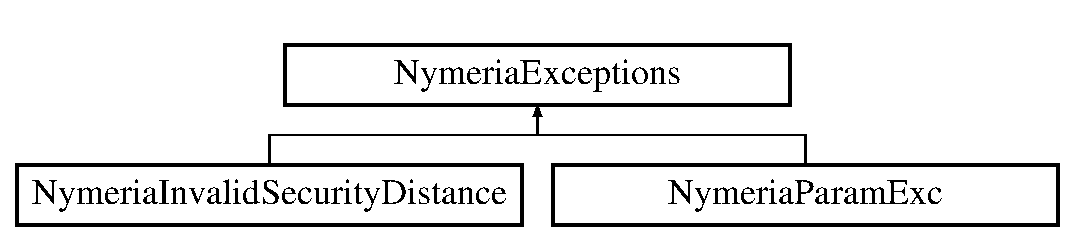
\includegraphics[height=2.000000cm]{classNymeriaExceptions}
\end{center}
\end{figure}
\subsection*{\-Public \-Member \-Functions}
\begin{DoxyCompactItemize}
\item 
\hypertarget{classNymeriaExceptions_a2ffc37214bfd0d77123c81e4d11f05c3}{{\bfseries \-Nymeria\-Exceptions} (string msg)}\label{classNymeriaExceptions_a2ffc37214bfd0d77123c81e4d11f05c3}

\item 
\hypertarget{classNymeriaExceptions_a3eb752e6b582566cec814e208294b4c6}{virtual const char $\ast$ {\bfseries what} () const   throw ()}\label{classNymeriaExceptions_a3eb752e6b582566cec814e208294b4c6}

\end{DoxyCompactItemize}


\subsection{\-Detailed \-Description}
\-Declaration of the class \hyperlink{classNymeriaExceptions}{\-Nymeria\-Exceptions}, that declares the base class for all exceptions particular to \hyperlink{classNymeria}{\-Nymeria}. 

\-The documentation for this class was generated from the following file\-:\begin{DoxyCompactItemize}
\item 
include/nymeria\-\_\-ardrone/\-Nymeria\-Exceptions.\-h\end{DoxyCompactItemize}

\hypertarget{classNymeriaInvalidSecurityDistance}{\section{\-Nymeria\-Invalid\-Security\-Distance \-Class \-Reference}
\label{classNymeriaInvalidSecurityDistance}\index{\-Nymeria\-Invalid\-Security\-Distance@{\-Nymeria\-Invalid\-Security\-Distance}}
}


{\ttfamily \#include $<$\-Nymeria\-Invalid\-Security\-Distance.\-h$>$}

\-Inheritance diagram for \-Nymeria\-Invalid\-Security\-Distance\-:\begin{figure}[H]
\begin{center}
\leavevmode
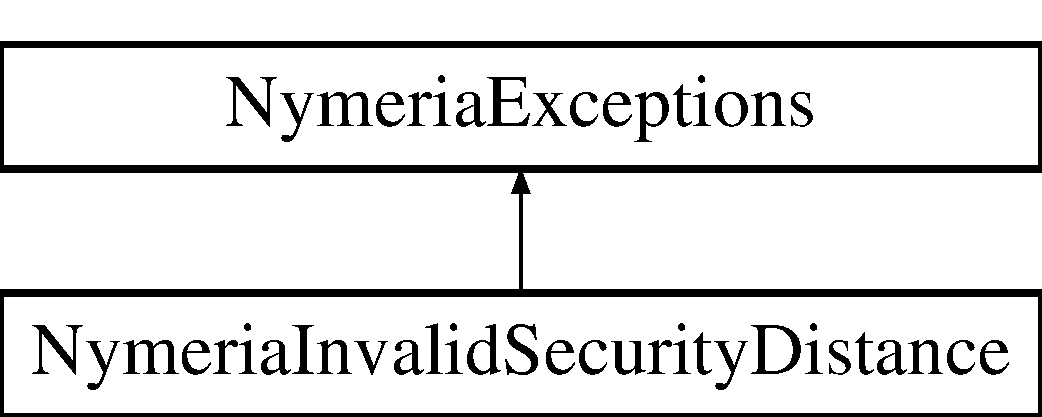
\includegraphics[height=2.000000cm]{classNymeriaInvalidSecurityDistance}
\end{center}
\end{figure}
\subsection*{\-Public \-Member \-Functions}
\begin{DoxyCompactItemize}
\item 
\hypertarget{classNymeriaInvalidSecurityDistance_adf2ed913aa00ca68f37c6eb794b161ca}{virtual const char $\ast$ {\bfseries what} () const   throw ()}\label{classNymeriaInvalidSecurityDistance_adf2ed913aa00ca68f37c6eb794b161ca}

\end{DoxyCompactItemize}


\subsection{\-Detailed \-Description}
\-Declaration of the class \hyperlink{classNymeriaParamExc}{\-Nymeria\-Param\-Exc}, that declares the exception thrown when the \-R\-O\-S parameter requested does not exist or was misspelled. 

\-The documentation for this class was generated from the following file\-:\begin{DoxyCompactItemize}
\item 
include/nymeria\-\_\-ardrone/\-Nymeria\-Invalid\-Security\-Distance.\-h\end{DoxyCompactItemize}

\hypertarget{classNymeriaMutex}{\section{\-Nymeria\-Mutex \-Class \-Reference}
\label{classNymeriaMutex}\index{\-Nymeria\-Mutex@{\-Nymeria\-Mutex}}
}
\-Inheritance diagram for \-Nymeria\-Mutex\-:\begin{figure}[H]
\begin{center}
\leavevmode
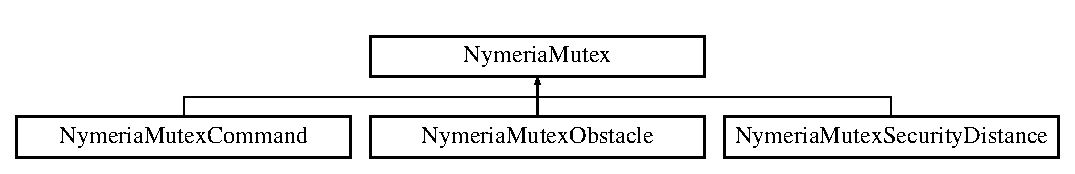
\includegraphics[height=1.895093cm]{classNymeriaMutex}
\end{center}
\end{figure}


\-The documentation for this class was generated from the following files\-:\begin{DoxyCompactItemize}
\item 
include/nymeria\-\_\-ardrone/\-Nymeria\-Mutex.\-h\item 
src/\-Nymeria\-Mutex.\-cpp\end{DoxyCompactItemize}

\hypertarget{classNymeriaMutexCommand}{\section{\-Nymeria\-Mutex\-Command \-Class \-Reference}
\label{classNymeriaMutexCommand}\index{\-Nymeria\-Mutex\-Command@{\-Nymeria\-Mutex\-Command}}
}
\-Inheritance diagram for \-Nymeria\-Mutex\-Command\-:\begin{figure}[H]
\begin{center}
\leavevmode
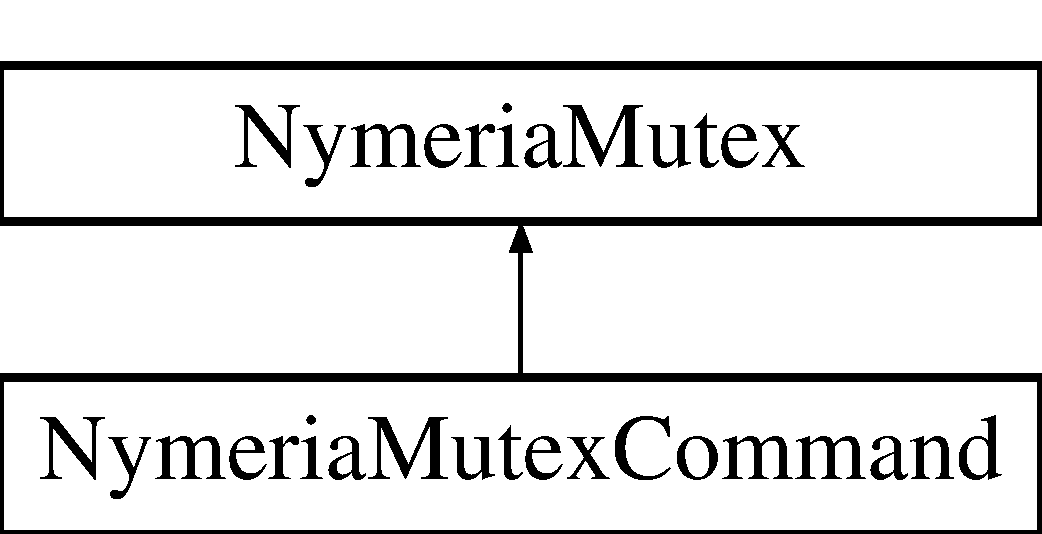
\includegraphics[height=2.000000cm]{classNymeriaMutexCommand}
\end{center}
\end{figure}
\subsection*{\-Static \-Public \-Member \-Functions}
\begin{DoxyCompactItemize}
\item 
\hypertarget{classNymeriaMutexCommand_a3aef40b73394ef9c59c30df348ad760c}{static \hyperlink{classNymeriaMutexCommand}{\-Nymeria\-Mutex\-Command} $\ast$ {\bfseries get\-Instance} ()}\label{classNymeriaMutexCommand_a3aef40b73394ef9c59c30df348ad760c}

\item 
\hypertarget{classNymeriaMutexCommand_a48016d42ec51705f59c774aa2dc19796}{static void {\bfseries lock} ()}\label{classNymeriaMutexCommand_a48016d42ec51705f59c774aa2dc19796}

\item 
\hypertarget{classNymeriaMutexCommand_afea66e700a433145efeafd9b8a53df7b}{static void {\bfseries unlock} ()}\label{classNymeriaMutexCommand_afea66e700a433145efeafd9b8a53df7b}

\end{DoxyCompactItemize}


\-The documentation for this class was generated from the following files\-:\begin{DoxyCompactItemize}
\item 
include/nymeria\-\_\-ardrone/\-Nymeria\-Mutex\-Command.\-h\item 
src/\-Nymeria\-Mutex\-Command.\-cpp\end{DoxyCompactItemize}

\hypertarget{classNymeriaMutexObstacle}{\section{\-Nymeria\-Mutex\-Obstacle \-Class \-Reference}
\label{classNymeriaMutexObstacle}\index{\-Nymeria\-Mutex\-Obstacle@{\-Nymeria\-Mutex\-Obstacle}}
}
\-Inheritance diagram for \-Nymeria\-Mutex\-Obstacle\-:\begin{figure}[H]
\begin{center}
\leavevmode
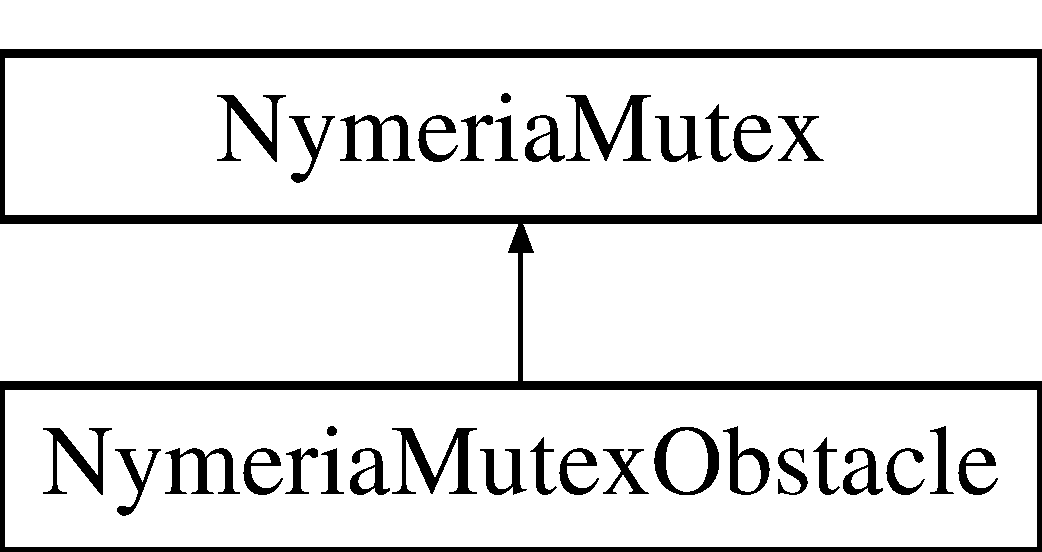
\includegraphics[height=2.000000cm]{classNymeriaMutexObstacle}
\end{center}
\end{figure}
\subsection*{\-Static \-Public \-Member \-Functions}
\begin{DoxyCompactItemize}
\item 
\hypertarget{classNymeriaMutexObstacle_a781305cfbe891eaf547c9d023b42d272}{static \hyperlink{classNymeriaMutexObstacle}{\-Nymeria\-Mutex\-Obstacle} $\ast$ {\bfseries get\-Instance} ()}\label{classNymeriaMutexObstacle_a781305cfbe891eaf547c9d023b42d272}

\item 
\hypertarget{classNymeriaMutexObstacle_ac9c77e3c39a6037aaf356d9d82460a40}{static void {\bfseries lock} ()}\label{classNymeriaMutexObstacle_ac9c77e3c39a6037aaf356d9d82460a40}

\item 
\hypertarget{classNymeriaMutexObstacle_ae10b2974844ac973a692be10eeaddf79}{static void {\bfseries unlock} ()}\label{classNymeriaMutexObstacle_ae10b2974844ac973a692be10eeaddf79}

\end{DoxyCompactItemize}


\-The documentation for this class was generated from the following files\-:\begin{DoxyCompactItemize}
\item 
include/nymeria\-\_\-ardrone/\-Nymeria\-Mutex\-Obstacle.\-h\item 
src/\-Nymeria\-Mutex\-Obstacle.\-cpp\end{DoxyCompactItemize}

\hypertarget{classNymeriaMutexSecurityDistance}{\section{\-Nymeria\-Mutex\-Security\-Distance \-Class \-Reference}
\label{classNymeriaMutexSecurityDistance}\index{\-Nymeria\-Mutex\-Security\-Distance@{\-Nymeria\-Mutex\-Security\-Distance}}
}
\-Inheritance diagram for \-Nymeria\-Mutex\-Security\-Distance\-:\begin{figure}[H]
\begin{center}
\leavevmode
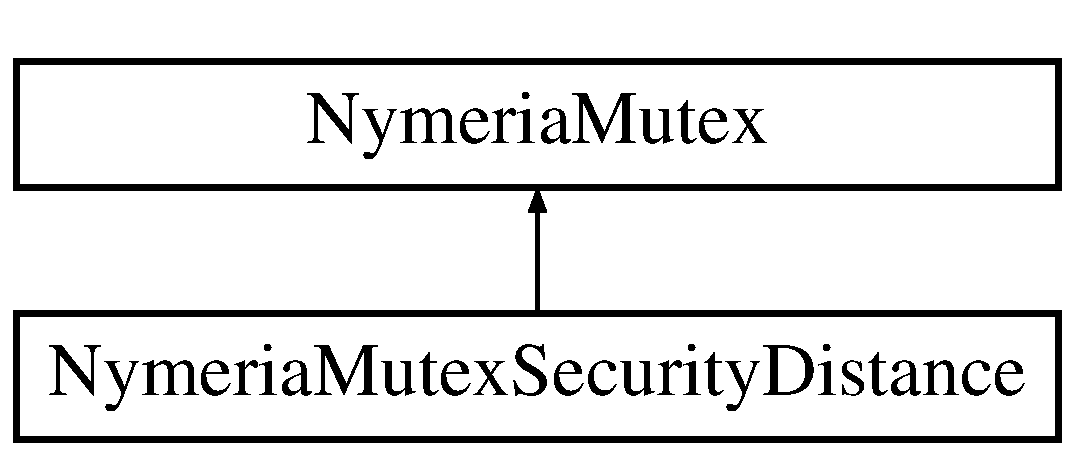
\includegraphics[height=2.000000cm]{classNymeriaMutexSecurityDistance}
\end{center}
\end{figure}
\subsection*{\-Static \-Public \-Member \-Functions}
\begin{DoxyCompactItemize}
\item 
\hypertarget{classNymeriaMutexSecurityDistance_a7de1c0314682fcdecf8e882eab57362b}{static \*
\hyperlink{classNymeriaMutexSecurityDistance}{\-Nymeria\-Mutex\-Security\-Distance} $\ast$ {\bfseries get\-Instance} ()}\label{classNymeriaMutexSecurityDistance_a7de1c0314682fcdecf8e882eab57362b}

\item 
\hypertarget{classNymeriaMutexSecurityDistance_a983390ed9dcef9b62c3df39f47e5bbe7}{static void {\bfseries lock} ()}\label{classNymeriaMutexSecurityDistance_a983390ed9dcef9b62c3df39f47e5bbe7}

\item 
\hypertarget{classNymeriaMutexSecurityDistance_a13d05cc109b0198a05091f0e2b108db5}{static void {\bfseries unlock} ()}\label{classNymeriaMutexSecurityDistance_a13d05cc109b0198a05091f0e2b108db5}

\end{DoxyCompactItemize}


\-The documentation for this class was generated from the following files\-:\begin{DoxyCompactItemize}
\item 
include/nymeria\-\_\-ardrone/\-Nymeria\-Mutex\-Security\-Distance.\-h\item 
src/\-Nymeria\-Mutex\-Security\-Distance.\-cpp\end{DoxyCompactItemize}

\hypertarget{classNymeriaParamExc}{\section{\-Nymeria\-Param\-Exc \-Class \-Reference}
\label{classNymeriaParamExc}\index{\-Nymeria\-Param\-Exc@{\-Nymeria\-Param\-Exc}}
}


{\ttfamily \#include $<$\-Nymeria\-Param\-Exc.\-h$>$}

\-Inheritance diagram for \-Nymeria\-Param\-Exc\-:\begin{figure}[H]
\begin{center}
\leavevmode
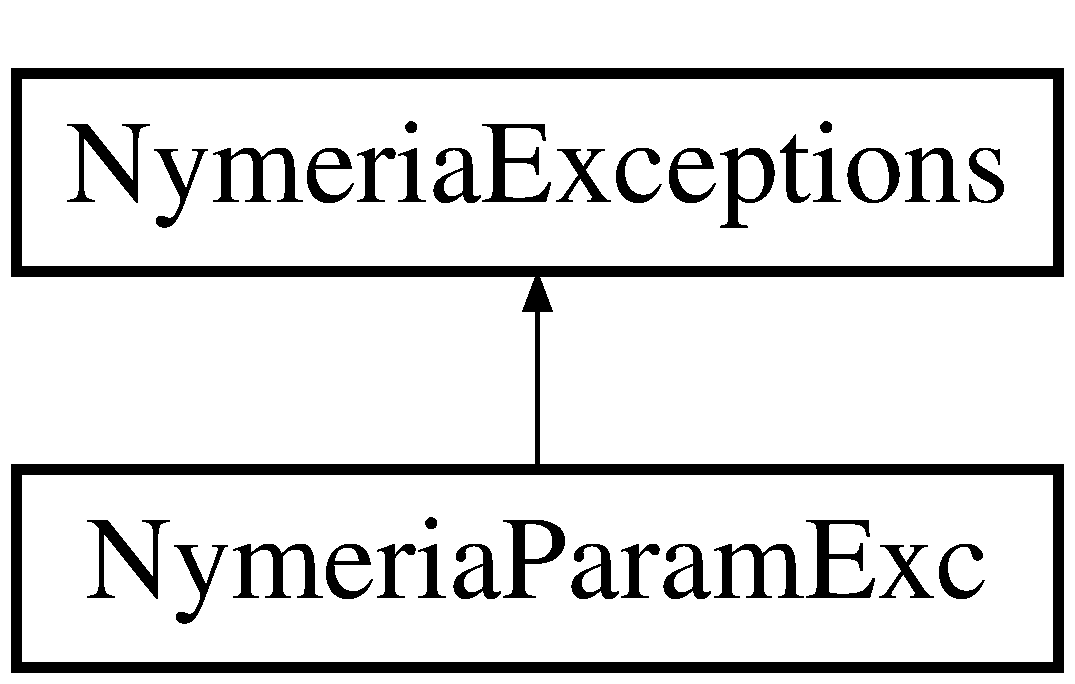
\includegraphics[height=2.000000cm]{classNymeriaParamExc}
\end{center}
\end{figure}
\subsection*{\-Public \-Member \-Functions}
\begin{DoxyCompactItemize}
\item 
\hypertarget{classNymeriaParamExc_a253c3cfe3e927036a1043836394cb6fe}{{\bfseries \-Nymeria\-Param\-Exc} (string msg=\char`\"{}\char`\"{})}\label{classNymeriaParamExc_a253c3cfe3e927036a1043836394cb6fe}

\item 
\hypertarget{classNymeriaParamExc_a7171011e1c64f0295f3eb3b5cec2b6da}{virtual const char $\ast$ {\bfseries what} () const   throw ()}\label{classNymeriaParamExc_a7171011e1c64f0295f3eb3b5cec2b6da}

\end{DoxyCompactItemize}


\subsection{\-Detailed \-Description}
\-Declaration of the class \hyperlink{classNymeriaParamExc}{\-Nymeria\-Param\-Exc}, that declares the exception thrown when the \-R\-O\-S parameter requested does not exist or was misspelled. 

\-The documentation for this class was generated from the following file\-:\begin{DoxyCompactItemize}
\item 
include/nymeria\-\_\-ardrone/\-Nymeria\-Param\-Exc.\-h\end{DoxyCompactItemize}

\hypertarget{classSensorInterface}{\section{\-Sensor\-Interface \-Class \-Reference}
\label{classSensorInterface}\index{\-Sensor\-Interface@{\-Sensor\-Interface}}
}
\subsection*{\-Public \-Member \-Functions}
\begin{DoxyCompactItemize}
\item 
\hypertarget{classSensorInterface_aeef00eab4b671a1f682a8caf91a97277}{void {\bfseries loop} (ros\-::\-Node\-Handle $\ast$n)}\label{classSensorInterface_aeef00eab4b671a1f682a8caf91a97277}

\item 
\hypertarget{classSensorInterface_aca7644c244097082ae20598ab7b428ea}{ros\-::\-Node\-Handle $\ast$ {\bfseries get\-N\-H} ()}\label{classSensorInterface_aca7644c244097082ae20598ab7b428ea}

\end{DoxyCompactItemize}


\-The documentation for this class was generated from the following files\-:\begin{DoxyCompactItemize}
\item 
include/nymeria\-\_\-ardrone/\-Sensor\-Interface.\-h\item 
src/\-Sensor\-Interface.\-cpp\end{DoxyCompactItemize}

\hypertarget{classTeleopKeyboard}{\section{\-Teleop\-Keyboard \-Class \-Reference}
\label{classTeleopKeyboard}\index{\-Teleop\-Keyboard@{\-Teleop\-Keyboard}}
}
\subsection*{\-Public \-Member \-Functions}
\begin{DoxyCompactItemize}
\item 
\hypertarget{classTeleopKeyboard_a7829c0739622fed59aa5e66e0828d97e}{void {\bfseries key\-Loop} (ros\-::\-Node\-Handle $\ast$n)}\label{classTeleopKeyboard_a7829c0739622fed59aa5e66e0828d97e}

\item 
\hypertarget{classTeleopKeyboard_adaa0990f75d0534dc7d41a01fd24db09}{ros\-::\-Node\-Handle $\ast$ {\bfseries get\-N\-H} ()}\label{classTeleopKeyboard_adaa0990f75d0534dc7d41a01fd24db09}

\end{DoxyCompactItemize}


\-The documentation for this class was generated from the following files\-:\begin{DoxyCompactItemize}
\item 
include/nymeria\-\_\-ardrone/\-Teleop\-Keyboard.\-h\item 
src/\-Teleop\-Keyboard.\-cpp\end{DoxyCompactItemize}

\hypertarget{classUDPClient}{\section{\-U\-D\-P\-Client \-Class \-Reference}
\label{classUDPClient}\index{\-U\-D\-P\-Client@{\-U\-D\-P\-Client}}
}
\subsection*{\-Public \-Member \-Functions}
\begin{DoxyCompactItemize}
\item 
\hypertarget{classUDPClient_a97e34fe6f6f17bab4bd031ea1b79de7c}{{\bfseries \-U\-D\-P\-Client} (const std\-::string \&addr, int port)}\label{classUDPClient_a97e34fe6f6f17bab4bd031ea1b79de7c}

\item 
\hypertarget{classUDPClient_a5ac1eddc517f62615fae91d5efea2cc8}{int {\bfseries get\-\_\-socket} () const }\label{classUDPClient_a5ac1eddc517f62615fae91d5efea2cc8}

\item 
\hypertarget{classUDPClient_a1704aa3773d5133d3dd27b4ab90d6ed7}{int {\bfseries get\-\_\-port} () const }\label{classUDPClient_a1704aa3773d5133d3dd27b4ab90d6ed7}

\item 
\hypertarget{classUDPClient_a9c447c882c46dcdd0ce449feea44fd5d}{std\-::string {\bfseries get\-\_\-addr} () const }\label{classUDPClient_a9c447c882c46dcdd0ce449feea44fd5d}

\item 
\hypertarget{classUDPClient_a1f1e12cba5f35d9436e64bc1784171f8}{int {\bfseries send} (const char $\ast$msg, size\-\_\-t size)}\label{classUDPClient_a1f1e12cba5f35d9436e64bc1784171f8}

\item 
\hypertarget{classUDPClient_a0d68aacc0fc4e1842885178c362e97d1}{int {\bfseries recv} (char $\ast$msg, size\-\_\-t max\-\_\-size)}\label{classUDPClient_a0d68aacc0fc4e1842885178c362e97d1}

\item 
\hypertarget{classUDPClient_a97e34fe6f6f17bab4bd031ea1b79de7c}{{\bfseries \-U\-D\-P\-Client} (const std\-::string \&addr, int port)}\label{classUDPClient_a97e34fe6f6f17bab4bd031ea1b79de7c}

\item 
\hypertarget{classUDPClient_a5ac1eddc517f62615fae91d5efea2cc8}{int {\bfseries get\-\_\-socket} () const }\label{classUDPClient_a5ac1eddc517f62615fae91d5efea2cc8}

\item 
\hypertarget{classUDPClient_a1704aa3773d5133d3dd27b4ab90d6ed7}{int {\bfseries get\-\_\-port} () const }\label{classUDPClient_a1704aa3773d5133d3dd27b4ab90d6ed7}

\item 
\hypertarget{classUDPClient_a9c447c882c46dcdd0ce449feea44fd5d}{std\-::string {\bfseries get\-\_\-addr} () const }\label{classUDPClient_a9c447c882c46dcdd0ce449feea44fd5d}

\item 
\hypertarget{classUDPClient_a1f1e12cba5f35d9436e64bc1784171f8}{int {\bfseries send} (const char $\ast$msg, size\-\_\-t size)}\label{classUDPClient_a1f1e12cba5f35d9436e64bc1784171f8}

\item 
\hypertarget{classUDPClient_a0d68aacc0fc4e1842885178c362e97d1}{int {\bfseries recv} (char $\ast$msg, size\-\_\-t max\-\_\-size)}\label{classUDPClient_a0d68aacc0fc4e1842885178c362e97d1}

\end{DoxyCompactItemize}


\-The documentation for this class was generated from the following files\-:\begin{DoxyCompactItemize}
\item 
include/nymeria\-\_\-ardrone/\-U\-D\-P\-Wrapper.\-h\item 
embedded/\-U\-D\-P\-Wrapper.\-h\item 
src/\-U\-D\-P\-Wrapper.\-cpp\item 
embedded/\-U\-D\-P\-Wrapper.\-cpp\end{DoxyCompactItemize}

\hypertarget{classUDPServer}{\section{\-U\-D\-P\-Server \-Class \-Reference}
\label{classUDPServer}\index{\-U\-D\-P\-Server@{\-U\-D\-P\-Server}}
}
\subsection*{\-Public \-Member \-Functions}
\begin{DoxyCompactItemize}
\item 
\hypertarget{classUDPServer_a1c329d510895a368942ade66e27ded41}{{\bfseries \-U\-D\-P\-Server} (const std\-::string \&addr, int port)}\label{classUDPServer_a1c329d510895a368942ade66e27ded41}

\item 
\hypertarget{classUDPServer_afa98d6638cc862fc150867b4a7399ae2}{int {\bfseries get\-\_\-socket} () const }\label{classUDPServer_afa98d6638cc862fc150867b4a7399ae2}

\item 
\hypertarget{classUDPServer_a3fd4e5a227d9b417bcbf8e88268d200a}{int {\bfseries get\-\_\-port} () const }\label{classUDPServer_a3fd4e5a227d9b417bcbf8e88268d200a}

\item 
\hypertarget{classUDPServer_a736dde370ce9eb0d474a5fad266111fb}{std\-::string {\bfseries get\-\_\-addr} () const }\label{classUDPServer_a736dde370ce9eb0d474a5fad266111fb}

\item 
\hypertarget{classUDPServer_a69e88e5fcdeee3f0e9c5fe3cdfba9a74}{int {\bfseries recv} (char $\ast$msg, size\-\_\-t max\-\_\-size)}\label{classUDPServer_a69e88e5fcdeee3f0e9c5fe3cdfba9a74}

\item 
\hypertarget{classUDPServer_ae8585a5e5fd62713a970be89a99498ee}{int {\bfseries send} (const char $\ast$msg, size\-\_\-t size)}\label{classUDPServer_ae8585a5e5fd62713a970be89a99498ee}

\item 
\hypertarget{classUDPServer_a59a89ed608c268960cafc460601dcb39}{int {\bfseries send} (const char $\ast$msg, size\-\_\-t size, const std\-::string \&addr, int port)}\label{classUDPServer_a59a89ed608c268960cafc460601dcb39}

\item 
\hypertarget{classUDPServer_a1c329d510895a368942ade66e27ded41}{{\bfseries \-U\-D\-P\-Server} (const std\-::string \&addr, int port)}\label{classUDPServer_a1c329d510895a368942ade66e27ded41}

\item 
\hypertarget{classUDPServer_afa98d6638cc862fc150867b4a7399ae2}{int {\bfseries get\-\_\-socket} () const }\label{classUDPServer_afa98d6638cc862fc150867b4a7399ae2}

\item 
\hypertarget{classUDPServer_a3fd4e5a227d9b417bcbf8e88268d200a}{int {\bfseries get\-\_\-port} () const }\label{classUDPServer_a3fd4e5a227d9b417bcbf8e88268d200a}

\item 
\hypertarget{classUDPServer_a736dde370ce9eb0d474a5fad266111fb}{std\-::string {\bfseries get\-\_\-addr} () const }\label{classUDPServer_a736dde370ce9eb0d474a5fad266111fb}

\item 
\hypertarget{classUDPServer_a69e88e5fcdeee3f0e9c5fe3cdfba9a74}{int {\bfseries recv} (char $\ast$msg, size\-\_\-t max\-\_\-size)}\label{classUDPServer_a69e88e5fcdeee3f0e9c5fe3cdfba9a74}

\item 
\hypertarget{classUDPServer_ae8585a5e5fd62713a970be89a99498ee}{int {\bfseries send} (const char $\ast$msg, size\-\_\-t size)}\label{classUDPServer_ae8585a5e5fd62713a970be89a99498ee}

\item 
\hypertarget{classUDPServer_a59a89ed608c268960cafc460601dcb39}{int {\bfseries send} (const char $\ast$msg, size\-\_\-t size, const std\-::string \&addr, int port)}\label{classUDPServer_a59a89ed608c268960cafc460601dcb39}

\end{DoxyCompactItemize}


\-The documentation for this class was generated from the following files\-:\begin{DoxyCompactItemize}
\item 
include/nymeria\-\_\-ardrone/\-U\-D\-P\-Wrapper.\-h\item 
embedded/\-U\-D\-P\-Wrapper.\-h\item 
src/\-U\-D\-P\-Wrapper.\-cpp\item 
embedded/\-U\-D\-P\-Wrapper.\-cpp\end{DoxyCompactItemize}

\chapter{\-File \-Documentation}
\hypertarget{Nymeria_8cpp}{\section{src/\-Nymeria.cpp \-File \-Reference}
\label{Nymeria_8cpp}\index{src/\-Nymeria.\-cpp@{src/\-Nymeria.\-cpp}}
}
{\ttfamily \#include $<$nymeria\-\_\-ardrone/\-Nymeria.\-h$>$}\*
{\ttfamily \#include $<$nymeria\-\_\-ardrone/\-Nymeria\-Param\-Exc.\-h$>$}\*
{\ttfamily \#include $<$nymeria\-\_\-ardrone/\-Nymeria\-Invalid\-Security\-Distance.\-h$>$}\*
{\ttfamily \#include $<$nymeria\-\_\-ardrone/\-Nymeria\-Mutex\-Command.\-h$>$}\*
{\ttfamily \#include $<$nymeria\-\_\-ardrone/\-Nymeria\-Mutex\-Obstacle.\-h$>$}\*
{\ttfamily \#include $<$nymeria\-\_\-ardrone/\-Nymeria\-Mutex\-Security\-Distance.\-h$>$}\*
{\ttfamily \#include $<$string.\-h$>$}\*


\subsection{\-Detailed \-Description}

\printindex
\end{document}
